\documentclass[tikz,border=10pt]{standalone}
% Shared style for all Speed Demon diagrams: one palette, rounded white boxes,
% dark ink, white page (readable on GitHub light and dark).
\hyphenpenalty=10000 \exhyphenpenalty=10000 \tolerance=9999
\usepackage[T1]{fontenc}
\usepackage[scaled=0.95]{helvet}
\renewcommand{\familydefault}{\sfdefault}
\usepackage{tikz}
\usepackage{pgfplots}
\pgfplotsset{compat=1.16}
\usetikzlibrary{arrows.meta,positioning,shapes.geometric,fit,backgrounds,calc}

\definecolor{ink}{HTML}{1F2937}
\definecolor{mute}{HTML}{6B7280}
\definecolor{rule}{HTML}{9CA3AF}
\definecolor{cA}{HTML}{2563EB}   % Track A  blue
\definecolor{cB}{HTML}{D97706}   % Track B  amber
\definecolor{cC}{HTML}{059669}   % Track C  green
\definecolor{cD}{HTML}{7C3AED}   % Track D  violet
\definecolor{warn}{HTML}{DC2626} % fallback / redo path
\definecolor{wash}{HTML}{F3F4F6}

\tikzset{
  every node/.style={font=\small, text=ink},
  >={Stealth[length=2.4mm,width=1.8mm]},
  box/.style={draw=ink, fill=white, rounded corners=3pt, line width=0.7pt,
    align=center, inner sep=5pt, minimum height=12mm, text width=#1},
  box/.default=44mm,
  accent/.style={draw=#1, line width=1.2pt},
  accent/.default=cA,
  hl/.style={fill=#1!10, draw=#1, line width=1.1pt},
  dec/.style={diamond, aspect=2.6, draw=ink, fill=white, line width=0.7pt,
    align=center, inner sep=2pt, text width=#1},
  dec/.default=34mm,
  arr/.style={->, line width=0.9pt, color=ink},
  redo/.style={->, line width=0.9pt, color=warn, dash pattern=on 4pt off 3pt},
  lab/.style={font=\footnotesize, text=mute, inner sep=2pt},
  grp/.style={draw=#1, dashed, line width=0.9pt, rounded corners=6pt, inner sep=9pt,
    fill=#1!4},
  grp/.default=mute,
  grplabel/.style={font=\footnotesize\bfseries, text=#1, inner sep=2pt},
  show background rectangle,
  background rectangle/.style={fill=white, rounded corners=0pt},
}
\pgfplotsset{
  every axis/.append style={font=\small, tick label style={font=\footnotesize},
    axis line style={ink}, tick style={ink}, grid style={rule!50},
    label style={font=\small}, title style={font=\small\bfseries}},
}

% node text: \nt{title}{detail}
\newcommand{\nt}[2]{\textbf{#1}\par\vspace{1pt}{\footnotesize #2}}

\begin{document}
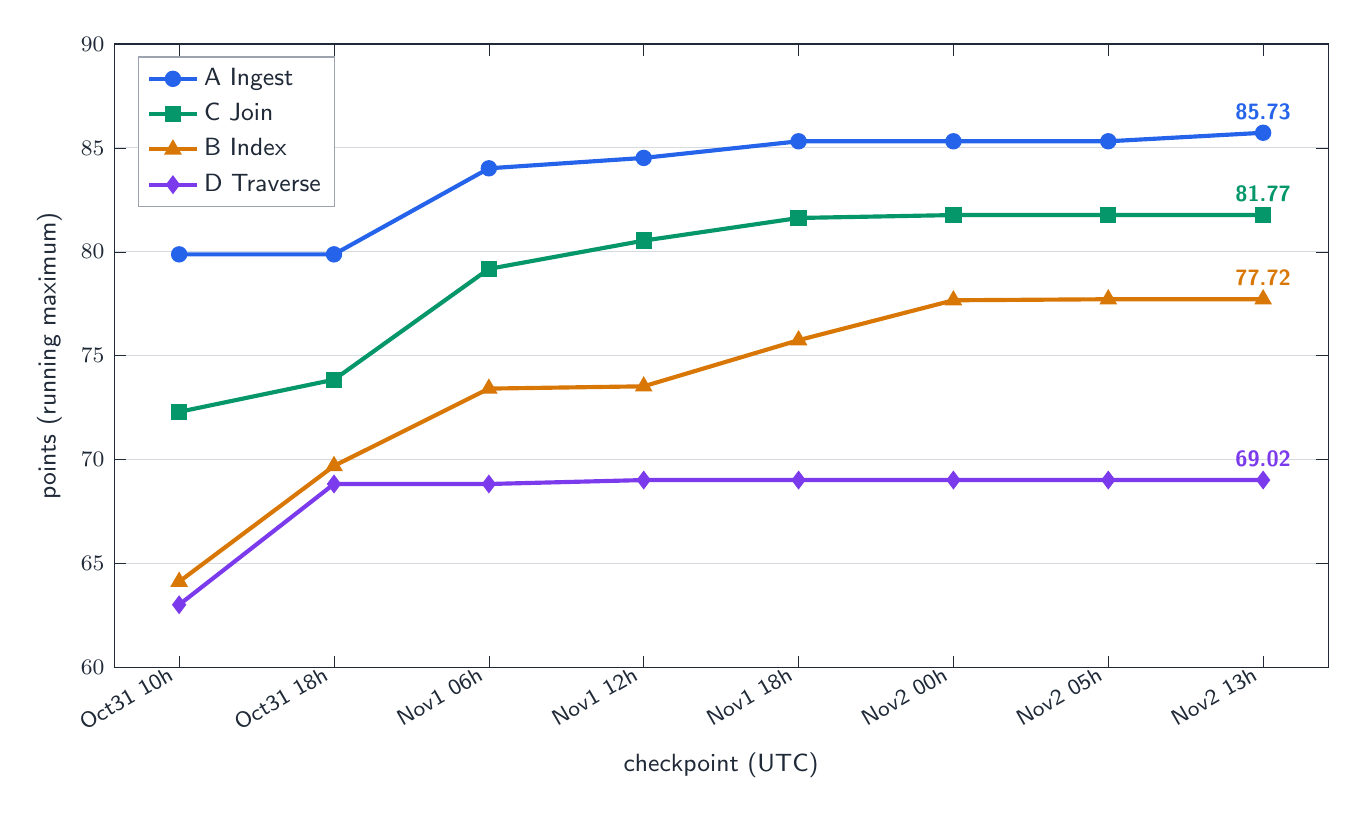
\begin{tikzpicture}
\begin{axis}[
  width=17cm, height=9.5cm,
  ymin=60, ymax=90, ytick distance=5,
  ylabel={points (running maximum)},
  symbolic x coords={Oct31 10h,Oct31 18h,Nov1 06h,Nov1 12h,Nov1 18h,Nov2 00h,Nov2 05h,Nov2 13h},
  xtick=data, x tick label style={rotate=30, anchor=east},
  xlabel={checkpoint (UTC)},
  ymajorgrids, grid style={rule!40},
  enlarge x limits=0.06,
  legend cell align=left, legend style={at={(0.02,0.98)}, anchor=north west, draw=rule, fill=white, font=\footnotesize, row sep=1pt},
  every axis plot/.append style={line width=1.5pt, mark size=2.2pt},
  clip=false,
]
\addplot[color=cA, mark=*] coordinates {(Oct31 10h,79.88) (Oct31 18h,79.88) (Nov1 06h,84.02) (Nov1 12h,84.52) (Nov1 18h,85.32) (Nov2 00h,85.32) (Nov2 05h,85.32) (Nov2 13h,85.73)};
\addplot[color=cC, mark=square*] coordinates {(Oct31 10h,72.30) (Oct31 18h,73.85) (Nov1 06h,79.18) (Nov1 12h,80.54) (Nov1 18h,81.63) (Nov2 00h,81.77) (Nov2 05h,81.77) (Nov2 13h,81.77)};
\addplot[color=cB, mark=triangle*] coordinates {(Oct31 10h,64.13) (Oct31 18h,69.70) (Nov1 06h,73.42) (Nov1 12h,73.53) (Nov1 18h,75.75) (Nov2 00h,77.67) (Nov2 05h,77.72) (Nov2 13h,77.72)};
\addplot[color=cD, mark=diamond*] coordinates {(Oct31 10h,63.02) (Oct31 18h,68.83) (Nov1 06h,68.83) (Nov1 12h,69.02) (Nov1 18h,69.02) (Nov2 00h,69.02) (Nov2 05h,69.02) (Nov2 13h,69.02)};
\legend{A Ingest, C Join, B Index, D Traverse}
\node[font=\footnotesize\bfseries, text=cA, anchor=south] at (axis cs:Nov2 13h,85.9) {85.73};
\node[font=\footnotesize\bfseries, text=cC, anchor=south] at (axis cs:Nov2 13h,81.94) {81.77};
\node[font=\footnotesize\bfseries, text=cB, anchor=south] at (axis cs:Nov2 13h,77.89) {77.72};
\node[font=\footnotesize\bfseries, text=cD, anchor=south] at (axis cs:Nov2 13h,69.19) {69.02};
\end{axis}
\end{tikzpicture}
\end{document}
